% Options for packages loaded elsewhere
\PassOptionsToPackage{unicode}{hyperref}
\PassOptionsToPackage{hyphens}{url}
%
\documentclass[
  11pt,
]{article}
\usepackage{lmodern}
\usepackage{amsmath}
\usepackage{ifxetex,ifluatex}
\ifnum 0\ifxetex 1\fi\ifluatex 1\fi=0 % if pdftex
  \usepackage[T1]{fontenc}
  \usepackage[utf8]{inputenc}
  \usepackage{textcomp} % provide euro and other symbols
  \usepackage{amssymb}
\else % if luatex or xetex
  \usepackage{unicode-math}
  \defaultfontfeatures{Scale=MatchLowercase}
  \defaultfontfeatures[\rmfamily]{Ligatures=TeX,Scale=1}
  \setmainfont[]{Times New Roman}
\fi
% Use upquote if available, for straight quotes in verbatim environments
\IfFileExists{upquote.sty}{\usepackage{upquote}}{}
\IfFileExists{microtype.sty}{% use microtype if available
  \usepackage[]{microtype}
  \UseMicrotypeSet[protrusion]{basicmath} % disable protrusion for tt fonts
}{}
\makeatletter
\@ifundefined{KOMAClassName}{% if non-KOMA class
  \IfFileExists{parskip.sty}{%
    \usepackage{parskip}
  }{% else
    \setlength{\parindent}{0pt}
    \setlength{\parskip}{6pt plus 2pt minus 1pt}}
}{% if KOMA class
  \KOMAoptions{parskip=half}}
\makeatother
\usepackage{xcolor}
\IfFileExists{xurl.sty}{\usepackage{xurl}}{} % add URL line breaks if available
\IfFileExists{bookmark.sty}{\usepackage{bookmark}}{\usepackage{hyperref}}
\hypersetup{
  pdftitle={Task 1},
  hidelinks,
  pdfcreator={LaTeX via pandoc}}
\urlstyle{same} % disable monospaced font for URLs
\usepackage[margin=1in]{geometry}
\usepackage{color}
\usepackage{fancyvrb}
\newcommand{\VerbBar}{|}
\newcommand{\VERB}{\Verb[commandchars=\\\{\}]}
\DefineVerbatimEnvironment{Highlighting}{Verbatim}{commandchars=\\\{\}}
% Add ',fontsize=\small' for more characters per line
\usepackage{framed}
\definecolor{shadecolor}{RGB}{248,248,248}
\newenvironment{Shaded}{\begin{snugshade}}{\end{snugshade}}
\newcommand{\AlertTok}[1]{\textcolor[rgb]{0.94,0.16,0.16}{#1}}
\newcommand{\AnnotationTok}[1]{\textcolor[rgb]{0.56,0.35,0.01}{\textbf{\textit{#1}}}}
\newcommand{\AttributeTok}[1]{\textcolor[rgb]{0.77,0.63,0.00}{#1}}
\newcommand{\BaseNTok}[1]{\textcolor[rgb]{0.00,0.00,0.81}{#1}}
\newcommand{\BuiltInTok}[1]{#1}
\newcommand{\CharTok}[1]{\textcolor[rgb]{0.31,0.60,0.02}{#1}}
\newcommand{\CommentTok}[1]{\textcolor[rgb]{0.56,0.35,0.01}{\textit{#1}}}
\newcommand{\CommentVarTok}[1]{\textcolor[rgb]{0.56,0.35,0.01}{\textbf{\textit{#1}}}}
\newcommand{\ConstantTok}[1]{\textcolor[rgb]{0.00,0.00,0.00}{#1}}
\newcommand{\ControlFlowTok}[1]{\textcolor[rgb]{0.13,0.29,0.53}{\textbf{#1}}}
\newcommand{\DataTypeTok}[1]{\textcolor[rgb]{0.13,0.29,0.53}{#1}}
\newcommand{\DecValTok}[1]{\textcolor[rgb]{0.00,0.00,0.81}{#1}}
\newcommand{\DocumentationTok}[1]{\textcolor[rgb]{0.56,0.35,0.01}{\textbf{\textit{#1}}}}
\newcommand{\ErrorTok}[1]{\textcolor[rgb]{0.64,0.00,0.00}{\textbf{#1}}}
\newcommand{\ExtensionTok}[1]{#1}
\newcommand{\FloatTok}[1]{\textcolor[rgb]{0.00,0.00,0.81}{#1}}
\newcommand{\FunctionTok}[1]{\textcolor[rgb]{0.00,0.00,0.00}{#1}}
\newcommand{\ImportTok}[1]{#1}
\newcommand{\InformationTok}[1]{\textcolor[rgb]{0.56,0.35,0.01}{\textbf{\textit{#1}}}}
\newcommand{\KeywordTok}[1]{\textcolor[rgb]{0.13,0.29,0.53}{\textbf{#1}}}
\newcommand{\NormalTok}[1]{#1}
\newcommand{\OperatorTok}[1]{\textcolor[rgb]{0.81,0.36,0.00}{\textbf{#1}}}
\newcommand{\OtherTok}[1]{\textcolor[rgb]{0.56,0.35,0.01}{#1}}
\newcommand{\PreprocessorTok}[1]{\textcolor[rgb]{0.56,0.35,0.01}{\textit{#1}}}
\newcommand{\RegionMarkerTok}[1]{#1}
\newcommand{\SpecialCharTok}[1]{\textcolor[rgb]{0.00,0.00,0.00}{#1}}
\newcommand{\SpecialStringTok}[1]{\textcolor[rgb]{0.31,0.60,0.02}{#1}}
\newcommand{\StringTok}[1]{\textcolor[rgb]{0.31,0.60,0.02}{#1}}
\newcommand{\VariableTok}[1]{\textcolor[rgb]{0.00,0.00,0.00}{#1}}
\newcommand{\VerbatimStringTok}[1]{\textcolor[rgb]{0.31,0.60,0.02}{#1}}
\newcommand{\WarningTok}[1]{\textcolor[rgb]{0.56,0.35,0.01}{\textbf{\textit{#1}}}}
\usepackage{longtable,booktabs}
\usepackage{calc} % for calculating minipage widths
% Correct order of tables after \paragraph or \subparagraph
\usepackage{etoolbox}
\makeatletter
\patchcmd\longtable{\par}{\if@noskipsec\mbox{}\fi\par}{}{}
\makeatother
% Allow footnotes in longtable head/foot
\IfFileExists{footnotehyper.sty}{\usepackage{footnotehyper}}{\usepackage{footnote}}
\makesavenoteenv{longtable}
\usepackage{graphicx}
\makeatletter
\def\maxwidth{\ifdim\Gin@nat@width>\linewidth\linewidth\else\Gin@nat@width\fi}
\def\maxheight{\ifdim\Gin@nat@height>\textheight\textheight\else\Gin@nat@height\fi}
\makeatother
% Scale images if necessary, so that they will not overflow the page
% margins by default, and it is still possible to overwrite the defaults
% using explicit options in \includegraphics[width, height, ...]{}
\setkeys{Gin}{width=\maxwidth,height=\maxheight,keepaspectratio}
% Set default figure placement to htbp
\makeatletter
\def\fps@figure{htbp}
\makeatother
\setlength{\emergencystretch}{3em} % prevent overfull lines
\providecommand{\tightlist}{%
  \setlength{\itemsep}{0pt}\setlength{\parskip}{0pt}}
\setcounter{secnumdepth}{5}
\usepackage[font=small,format=plain,labelfont=bf,up,textfont=normal,up,justification=justified,singlelinecheck=false]{caption}
\usepackage{booktabs}
\usepackage{longtable}
\usepackage{array}
\usepackage{multirow}
\usepackage{wrapfig}
\usepackage{float}
\usepackage{colortbl}
\usepackage{pdflscape}
\usepackage{tabu}
\usepackage{threeparttable}
\usepackage{threeparttablex}
\usepackage[normalem]{ulem}
\usepackage{makecell}
\usepackage{xcolor}
\ifluatex
  \usepackage{selnolig}  % disable illegal ligatures
\fi

\title{Task 1}
\author{}
\date{\vspace{-2.5em}}

\begin{document}
\maketitle

{
\setcounter{tocdepth}{2}
\tableofcontents
}
\hypertarget{introduction}{%
\section{Introduction}\label{introduction}}

In the present part of the report, we will investigate to what extent we will be able to classify respondents in their country, and then we will compare the performance of different classifiers.

\hypertarget{data}{%
\section{Data}\label{data}}

The data have been obtained from the \(6^{th}\) Wave of the World Value Survey, which was carried out between 2010 and 2013. The data include the standardized scores of 3929 respondents of 3 countries on 32 variables, that have been summarized with 7 factors obtained using exploratory factor analysis with oblique rotation.
The 7 factors related to the 32 variables are:

\begin{enumerate}
\def\labelenumi{\arabic{enumi}.}
\tightlist
\item
  \textbf{Rights}, that it's related to homosexuality, prostitution, abortion, divorce, sex before marriage, suicide;
\item
  \textbf{Steal}, that it's related to claiming benefits, avoiding fare, stealing property, cheating taxes, accept a bribe;
\item
  \textbf{Crime}, that it's related to robberies, alcohol, police-military, racist behavior, drug sale;
\item
  \textbf{Religion}, that it's related to attend religious services, pray, the importance of God;
\item
  \textbf{Realize self}, that it's related to creative, rich, spoil oneself, be successful, exciting life;
\item
  \textbf{Do good}, that it's related to security, do good, behave properly, protect environment, tradition;
\item
  \textbf{Violence}, that it's related to beat wife, parents beating children, violenc.
\end{enumerate}

\hypertarget{methodology}{%
\section{Methodology}\label{methodology}}

To investigate the possibility to classify the respondents in their country based on the \(7\) factors we have used the canonical discriminant analysis. We have applied the linear regression function with \(7\) predictors and \(1\) dependent variable, the Country. Then to the output, we have applied the Canonical Discriminant Analysis.

\begin{Shaded}
\begin{Highlighting}[]
\NormalTok{lm.out}\OtherTok{\textless{}{-}}\FunctionTok{lm}\NormalTok{(}\FunctionTok{cbind}\NormalTok{(F\_rights, F\_steal, F\_crime,F\_religion,F\_realizeself,F\_dogood,}
\NormalTok{                 F\_violence)}\SpecialCharTok{\textasciitilde{}}\FunctionTok{as.factor}\NormalTok{(country), }\AttributeTok{data=}\NormalTok{dwvs)}
\NormalTok{candisc.out}\OtherTok{\textless{}{-}}\FunctionTok{candisc}\NormalTok{(lm.out)}
\FunctionTok{print}\NormalTok{(candisc.out)}
\end{Highlighting}
\end{Shaded}

\begin{verbatim}
Canonical Discriminant Analysis for as.factor(country):

   CanRsq Eigenvalue Difference Percent Cumulative
1 0.80691    4.17882     3.5622  87.142     87.142
2 0.38142    0.61661     3.5622  12.858    100.000

Test of H0: The canonical correlations in the 
current row and all that follow are zero

  LR test stat approx F numDF denDF   Pr(> F)    
1      0.11944  1059.53    14  7834 < 2.2e-16 ***
2      0.61858   402.65     6  3918 < 2.2e-16 ***
---
Signif. codes:  0 '***' 0.001 '**' 0.01 '*' 0.05 '.' 0.1 ' ' 1
\end{verbatim}

As we can see both the Square Canonical Correlation are significant, but the discriminating power to separate between the groups is higher for the first than for the second discriminant function: \(0.81\) and \(0.38\) respectively.
The LR test indicates that the discriminant analysis is meaningful. The first test's null hypothesis is \(H_{0}: \lambda_{1}=\lambda_{2}=0\) and this hypothesis as we can see from the \emph{p-value} is rejected. The \(null\) hypothesis of the first test it's equivalent to the test for \(H_{0}: \mu Netherlands = \mu Nigeria = \mu Philippines\).

The second LR test indicates that \(H_{0}:\lambda_{2}=0\), and also this null hypothesis is rejected. So even if the second discriminant function has less discriminant power cannot be omitted and it's statistically meaningful.

On our analysis, we have also applied two different tests for centroids and to test the equal covariance.

To see if the three-country has different centroids and confirm the results of the canonical discriminant analysis we have applied on the linear
regression the function \emph{Manova}:

\begin{Shaded}
\begin{Highlighting}[]
\NormalTok{res\_t1\_2 }\OtherTok{\textless{}{-}} \FunctionTok{summary}\NormalTok{(}\FunctionTok{Manova}\NormalTok{(lm.out), }\AttributeTok{test=}\StringTok{"Wilks"}\NormalTok{)}

\FunctionTok{summary.default}\NormalTok{(}\FunctionTok{Manova}\NormalTok{(lm.out), }\AttributeTok{test=}\StringTok{"Wilks"}\NormalTok{)}
\end{Highlighting}
\end{Shaded}

\begin{verbatim}
         Length Class  Mode     
SSP       1     -none- list     
SSPE     49     -none- numeric  
df        1     -none- numeric  
error.df  1     -none- numeric  
terms     1     -none- character
repeated  1     -none- logical  
type      1     -none- character
test      1     -none- character
\end{verbatim}

The \emph{p-value} is small, and the test confirms that the analysis is meaningful and that at least there is a pair of centroids that differs significantly. The function \emph{Manova} in r doing the \emph{Wilks Lambda test} uses the Rao approximation.
To test the assumption on equal population covariance we have applied to the linear regression the function \emph{boxM}:

\begin{Shaded}
\begin{Highlighting}[]
\FunctionTok{boxM}\NormalTok{(lm.out)}
\end{Highlighting}
\end{Shaded}

\begin{verbatim}
    Box's M-test for Homogeneity of Covariance Matrices

data:  Y
Chi-Sq (approx.) = 5479.2, df = 56, p-value < 2.2e-16
\end{verbatim}

The test of Box indicates that \(H_{0}\) of equal covariance matrices across groups is not supported by data.

\newpage

\hypertarget{plot}{%
\subsection{Plot}\label{plot}}

To complete the Canonical Discriminant analysis, we have plotted the three countries and the \(7\) variables.

\begin{verbatim}
Vector scale factor set to 7.827
\end{verbatim}

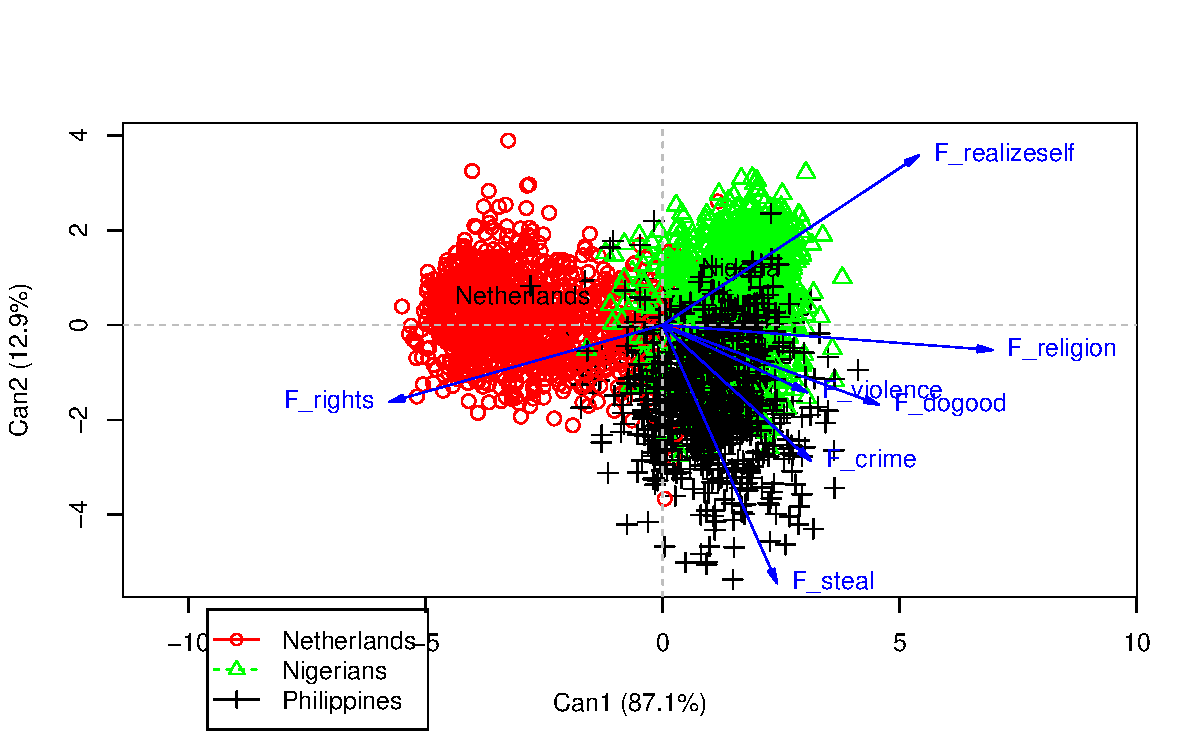
\includegraphics{1_Task_files/figure-latex/Task_1_4-1.pdf}

We can see that the group of individuals in \emph{red} are Netherlands citizens, the group of individuals in \emph{green} are Nigerians citizens and the group of individuals in \emph{black} are Philippines citizens. In blue we can see the \(7\) explanatory variables. The plot shows a clear separation between Netherlands and the other two countries on the first discriminant function while the second discriminant function could help to separate Nigeria and the Philippines.
The first discriminant function especially correlates with the factors: rights, religion, realize self, and do good; whereas the second discriminant function correlates with the factors: steal and realize self. The two-factor crime and violence have a lower correlation on the two factors and so has in this analysis lower importance on separate the \(3\) countries.

\hypertarget{compare-the-performance-of-different-classifiers}{%
\subsection{Compare the performance of different classifiers}\label{compare-the-performance-of-different-classifiers}}

We are going now to compare the performance of different classifiers to classify respondents in their country based on the \(7\) factors. To be able to do that we are going to compute the training error and the leave-one-out cross-validation error.
The classification method that we are going to compare are:
- Linear discriminant analysis;
- Quadratic discriminant analysis;
- K-nearest neighbors with k ranging from \emph{1 to 100};
- High Dimensional Discriminant Analysis;

\hypertarget{linear-discriminant-analysis}{%
\subsection{Linear discriminant analysis}\label{linear-discriminant-analysis}}

This method aims to separate in the clearest possible way different groups using the linear combination of observed independent variables. The linear discriminant analysis method assumes that the covariance structure of the independent variable is the same across groups. In our analysis, we know from the Box test previously computed that this assumption is not supported by the data. It will be an interesting test if in this case the Quadratic discriminant analysis, where the assumption on the equality of covariance matrix is relaxed, will perform better.
In the linear discriminant analysis, we have applied the method of Fisher correcting for the different prior probability.

\begin{Shaded}
\begin{Highlighting}[]
\NormalTok{lda.out1}\OtherTok{\textless{}{-}}\FunctionTok{lda}\NormalTok{(country }\SpecialCharTok{\textasciitilde{}}\NormalTok{ F\_rights }\SpecialCharTok{+}\NormalTok{ F\_steal }\SpecialCharTok{+}\NormalTok{ F\_crime }\SpecialCharTok{+}\NormalTok{ F\_religion }\SpecialCharTok{+}\NormalTok{ F\_realizeself }\SpecialCharTok{+}
\NormalTok{                F\_dogood }\SpecialCharTok{+}\NormalTok{ F\_violence, }\AttributeTok{data=}\NormalTok{dwvs)}
\CommentTok{\#print(lda.out1)}
\NormalTok{pred.train1 }\OtherTok{\textless{}{-}} \FunctionTok{predict}\NormalTok{(lda.out1,dwvs, }\AttributeTok{prior=}\FunctionTok{c}\NormalTok{(}\DecValTok{1}\NormalTok{,}\DecValTok{1}\NormalTok{,}\DecValTok{1}\NormalTok{)}\SpecialCharTok{/}\DecValTok{3}\NormalTok{)}
\end{Highlighting}
\end{Shaded}

\begin{Shaded}
\begin{Highlighting}[]
\NormalTok{tab1 }\OtherTok{\textless{}{-}} \FunctionTok{table}\NormalTok{(dwvs}\SpecialCharTok{$}\NormalTok{country,pred.train1}\SpecialCharTok{$}\NormalTok{class)}
\CommentTok{\#print(tab1)}
\FunctionTok{kbl}\NormalTok{(tab1)}
\end{Highlighting}
\end{Shaded}

\begin{tabular}[t]{l|r|r|r}
\hline
  & Netherlands & Nigeria & Philippines\\
\hline
Netherlands & 1145 & 39 & 76\\
\hline
Nigeria & 10 & 1327 & 241\\
\hline
Philippines & 17 & 220 & 851\\
\hline
\end{tabular}

\begin{Shaded}
\begin{Highlighting}[]
\CommentTok{\#training hit rate}
\FunctionTok{kbl}\NormalTok{(}\FunctionTok{sum}\NormalTok{(}\FunctionTok{diag}\NormalTok{(tab1))}\SpecialCharTok{/}\FunctionTok{sum}\NormalTok{(tab1))}
\end{Highlighting}
\end{Shaded}

\begin{tabular}[t]{r}
\hline
x\\
\hline
0.8464086\\
\hline
\end{tabular}

\begin{Shaded}
\begin{Highlighting}[]
\CommentTok{\#classify test observations using LDA}
\NormalTok{pred.loocv2}\OtherTok{\textless{}{-}}\FunctionTok{lda}\NormalTok{(country}\SpecialCharTok{\textasciitilde{}}\NormalTok{F\_rights}\SpecialCharTok{+}\NormalTok{F\_steal}\SpecialCharTok{+}\NormalTok{F\_crime}\SpecialCharTok{+}\NormalTok{F\_religion}\SpecialCharTok{+}\NormalTok{F\_realizeself}\SpecialCharTok{+}\NormalTok{F\_dogood}\SpecialCharTok{+}
\NormalTok{                   F\_violence,}\AttributeTok{data=}\NormalTok{dwvs, }\AttributeTok{prior=}\FunctionTok{c}\NormalTok{(}\DecValTok{1}\NormalTok{,}\DecValTok{1}\NormalTok{,}\DecValTok{1}\NormalTok{)}\SpecialCharTok{/}\DecValTok{3}\NormalTok{, }\AttributeTok{CV=}\ConstantTok{TRUE}\NormalTok{)}
\NormalTok{tab2}\OtherTok{\textless{}{-}}\FunctionTok{table}\NormalTok{(dwvs}\SpecialCharTok{$}\NormalTok{country,pred.loocv2}\SpecialCharTok{$}\NormalTok{class)}
\FunctionTok{print}\NormalTok{(tab2)}
\end{Highlighting}
\end{Shaded}

\begin{verbatim}
             
              Netherlands Nigeria Philippines
  Netherlands        1145      39          76
  Nigeria              11    1326         241
  Philippines          17     224         847
\end{verbatim}

\begin{Shaded}
\begin{Highlighting}[]
\CommentTok{\#LOOCV hit rate}
\FunctionTok{kbl}\NormalTok{(}\FunctionTok{sum}\NormalTok{(}\FunctionTok{diag}\NormalTok{(tab2))}\SpecialCharTok{/}\FunctionTok{sum}\NormalTok{(tab2))}
\end{Highlighting}
\end{Shaded}

\begin{tabular}[t]{r}
\hline
x\\
\hline
0.845135\\
\hline
\end{tabular}

We can see that in that case, the difference between the performance for training error and LOOCV error is really small, so there is no evidence for overfitting.

\hypertarget{quadratic-discriminant-analysis}{%
\subsection{Quadratic discriminant analysis}\label{quadratic-discriminant-analysis}}

The second method that we have applied is Quadratic discriminant analysis. It should perform better considering the difference in the covariance matrix for the different groups. QDA even if has a lower bias with a different covariance matrix, has a larger variance, and as in our case with a small dataset can be problematic.

Even in this case, we have applied the method of Fisher correcting for prior probabilities.

\begin{Shaded}
\begin{Highlighting}[]
\NormalTok{qda.out3}\OtherTok{\textless{}{-}}\FunctionTok{qda}\NormalTok{(country }\SpecialCharTok{\textasciitilde{}}\NormalTok{ F\_rights }\SpecialCharTok{+}\NormalTok{ F\_steal }\SpecialCharTok{+}\NormalTok{ F\_crime }\SpecialCharTok{+}\NormalTok{ F\_religion }\SpecialCharTok{+}\NormalTok{ F\_realizeself }\SpecialCharTok{+} 
\NormalTok{                F\_dogood }\SpecialCharTok{+}\NormalTok{ F\_violence, }\AttributeTok{data =}\NormalTok{ dwvs) }

\NormalTok{pred.train3}\OtherTok{\textless{}{-}}\FunctionTok{predict}\NormalTok{(qda.out3,dwvs, }\AttributeTok{prior=}\FunctionTok{c}\NormalTok{(}\DecValTok{1}\NormalTok{,}\DecValTok{1}\NormalTok{,}\DecValTok{1}\NormalTok{)}\SpecialCharTok{/}\DecValTok{3}\NormalTok{)}

\NormalTok{tab3}\OtherTok{\textless{}{-}}\FunctionTok{table}\NormalTok{(dwvs}\SpecialCharTok{$}\NormalTok{country,pred.train3}\SpecialCharTok{$}\NormalTok{class)}
\CommentTok{\#print(tab3)}
\FunctionTok{kbl}\NormalTok{(tab3)}
\end{Highlighting}
\end{Shaded}

\begin{tabular}[t]{l|r|r|r}
\hline
  & Netherlands & Nigeria & Philippines\\
\hline
Netherlands & 1210 & 21 & 29\\
\hline
Nigeria & 40 & 1319 & 219\\
\hline
Philippines & 41 & 219 & 828\\
\hline
\end{tabular}

\begin{Shaded}
\begin{Highlighting}[]
\CommentTok{\#training hit rate}
\FunctionTok{kbl}\NormalTok{(}\FunctionTok{sum}\NormalTok{(}\FunctionTok{diag}\NormalTok{(tab3))}\SpecialCharTok{/}\FunctionTok{sum}\NormalTok{(tab3))}
\end{Highlighting}
\end{Shaded}

\begin{tabular}[t]{r}
\hline
x\\
\hline
0.8550688\\
\hline
\end{tabular}

\begin{Shaded}
\begin{Highlighting}[]
\CommentTok{\#classify test observations using QDA}
\NormalTok{pred.test4 }\OtherTok{\textless{}{-}} \FunctionTok{qda}\NormalTok{(country }\SpecialCharTok{\textasciitilde{}}\NormalTok{ F\_rights }\SpecialCharTok{+}\NormalTok{ F\_steal }\SpecialCharTok{+}\NormalTok{ F\_crime }\SpecialCharTok{+}\NormalTok{ F\_religion }\SpecialCharTok{+}\NormalTok{ F\_realizeself }\SpecialCharTok{+} 
\NormalTok{                    F\_dogood }\SpecialCharTok{+}\NormalTok{ F\_violence, }\AttributeTok{data=}\NormalTok{dwvs,}\AttributeTok{prior=}\FunctionTok{c}\NormalTok{(}\DecValTok{1}\NormalTok{,}\DecValTok{1}\NormalTok{,}\DecValTok{1}\NormalTok{)}\SpecialCharTok{/}\DecValTok{3}\NormalTok{,}\AttributeTok{CV=}\ConstantTok{TRUE}\NormalTok{)}
\NormalTok{tab4}\OtherTok{\textless{}{-}}\FunctionTok{table}\NormalTok{(dwvs}\SpecialCharTok{$}\NormalTok{country,pred.test4}\SpecialCharTok{$}\NormalTok{class)}
\CommentTok{\#print(tab4)}
\FunctionTok{kbl}\NormalTok{(tab4)}
\end{Highlighting}
\end{Shaded}

\begin{tabular}[t]{l|r|r|r}
\hline
  & Netherlands & Nigeria & Philippines\\
\hline
Netherlands & 1210 & 21 & 29\\
\hline
Nigeria & 40 & 1315 & 223\\
\hline
Philippines & 43 & 223 & 822\\
\hline
\end{tabular}

\begin{Shaded}
\begin{Highlighting}[]
\CommentTok{\#LOOCV hit rate}
\FunctionTok{kbl}\NormalTok{(}\FunctionTok{sum}\NormalTok{(}\FunctionTok{diag}\NormalTok{(tab4))}\SpecialCharTok{/}\FunctionTok{sum}\NormalTok{(tab4))}
\end{Highlighting}
\end{Shaded}

\begin{tabular}[t]{r}
\hline
x\\
\hline
0.8525217\\
\hline
\end{tabular}

In that case there is also no evidence of overfitting. We can see from the results that the QDA performs better than the LDA but not with a significant improvement.

\hypertarget{k-nearest-neighbors}{%
\subsection{K-nearest Neighbors}\label{k-nearest-neighbors}}

The third model that we had analyzed is the K-nearest Neighbors. We have computed the model using all the 3926 observations, and to choose which is the correct number k of parameters to use, we have compared the training error with the Leave one out cross-validation error.

\begin{Shaded}
\begin{Highlighting}[]
\CommentTok{\#str(dwvs)}
\FunctionTok{table}\NormalTok{(dwvs}\SpecialCharTok{$}\NormalTok{country)}
\end{Highlighting}
\end{Shaded}

\begin{verbatim}
Netherlands     Nigeria Philippines 
       1260        1578        1088 
\end{verbatim}

\begin{Shaded}
\begin{Highlighting}[]
\FunctionTok{set.seed}\NormalTok{(}\DecValTok{9850}\NormalTok{)   }\CommentTok{\# {-}\textgreater{} random number generator}
\NormalTok{gp}\OtherTok{\textless{}{-}}\FunctionTok{runif}\NormalTok{(}\FunctionTok{nrow}\NormalTok{(dwvs))}
\NormalTok{dwvs2}\OtherTok{\textless{}{-}}\NormalTok{dwvs[}\FunctionTok{order}\NormalTok{(gp),]}
\CommentTok{\#str(dwvs)}
\CommentTok{\#str(dwvs2)}
\CommentTok{\#head(dwvs)}
\CommentTok{\#head(dwvs2)}

\NormalTok{hitratknn}\OtherTok{\textless{}{-}}\ControlFlowTok{function}\NormalTok{(observed,predicted)\{}
\NormalTok{  tab}\OtherTok{\textless{}{-}}\FunctionTok{table}\NormalTok{(observed,predicted)}
\NormalTok{  hitratknn}\OtherTok{\textless{}{-}}\FunctionTok{sum}\NormalTok{(}\FunctionTok{diag}\NormalTok{(tab))}\SpecialCharTok{/}\FunctionTok{sum}\NormalTok{(tab)}
  \FunctionTok{return}\NormalTok{(hitratknn)}
\NormalTok{\}}

\NormalTok{knnmax}\OtherTok{\textless{}{-}}\DecValTok{100}
\NormalTok{err}\OtherTok{\textless{}{-}}\FunctionTok{matrix}\NormalTok{(}\FunctionTok{rep}\NormalTok{(}\DecValTok{0}\NormalTok{,knnmax}\SpecialCharTok{*}\DecValTok{2}\NormalTok{), }\AttributeTok{nrow=}\NormalTok{knnmax)}

\ControlFlowTok{for}\NormalTok{(j }\ControlFlowTok{in} \DecValTok{1}\SpecialCharTok{:}\NormalTok{knnmax) \{}
\NormalTok{  predknn.train}\OtherTok{\textless{}{-}}\FunctionTok{knn}\NormalTok{(dwvs2[,}\DecValTok{2}\SpecialCharTok{:}\DecValTok{8}\NormalTok{], dwvs2[,}\DecValTok{2}\SpecialCharTok{:}\DecValTok{8}\NormalTok{], dwvs2}\SpecialCharTok{$}\NormalTok{country, }\AttributeTok{k=}\NormalTok{j)}
\NormalTok{  err[j,}\DecValTok{1}\NormalTok{]}\OtherTok{\textless{}{-}}\FunctionTok{hitratknn}\NormalTok{(dwvs2}\SpecialCharTok{$}\NormalTok{country,predknn.train)}
\NormalTok{\}}

\ControlFlowTok{for}\NormalTok{(j }\ControlFlowTok{in} \DecValTok{1}\SpecialCharTok{:}\NormalTok{knnmax) \{}
\NormalTok{  predknn.train}\OtherTok{\textless{}{-}}\FunctionTok{knn.cv}\NormalTok{(dwvs2[,}\DecValTok{2}\SpecialCharTok{:}\DecValTok{8}\NormalTok{], dwvs2}\SpecialCharTok{$}\NormalTok{country, }\AttributeTok{k=}\NormalTok{j)}
\NormalTok{  err [j,}\DecValTok{2}\NormalTok{]}\OtherTok{\textless{}{-}}\FunctionTok{hitratknn}\NormalTok{(dwvs2}\SpecialCharTok{$}\NormalTok{country,predknn.train)}
\NormalTok{\}}

\FunctionTok{plot}\NormalTok{(}\StringTok{\textquotesingle{}K\textquotesingle{}}\NormalTok{, }\StringTok{\textquotesingle{}Hit rate\textquotesingle{}}\NormalTok{,}\AttributeTok{xlim=}\FunctionTok{c}\NormalTok{(}\DecValTok{1}\NormalTok{,knnmax),}\AttributeTok{ylim=}\FunctionTok{c}\NormalTok{(}\FloatTok{0.8}\NormalTok{,}\DecValTok{1}\NormalTok{))}
\end{Highlighting}
\end{Shaded}

\begin{verbatim}
Warning in xy.coords(x, y, xlabel, ylabel, log): NAs introduced by coercion

Warning in xy.coords(x, y, xlabel, ylabel, log): NAs introduced by coercion
\end{verbatim}

\begin{Shaded}
\begin{Highlighting}[]
\FunctionTok{lines}\NormalTok{(}\FunctionTok{c}\NormalTok{(}\DecValTok{1}\SpecialCharTok{:}\NormalTok{knnmax),err[,}\DecValTok{1}\NormalTok{],}\AttributeTok{col=}\StringTok{"red"}\NormalTok{) }\CommentTok{\# {-}\textgreater{} training error}
\FunctionTok{lines}\NormalTok{(}\FunctionTok{c}\NormalTok{(}\DecValTok{1}\SpecialCharTok{:}\NormalTok{knnmax),err[,}\DecValTok{2}\NormalTok{],}\AttributeTok{col=}\StringTok{"blue"}\NormalTok{)}
\end{Highlighting}
\end{Shaded}

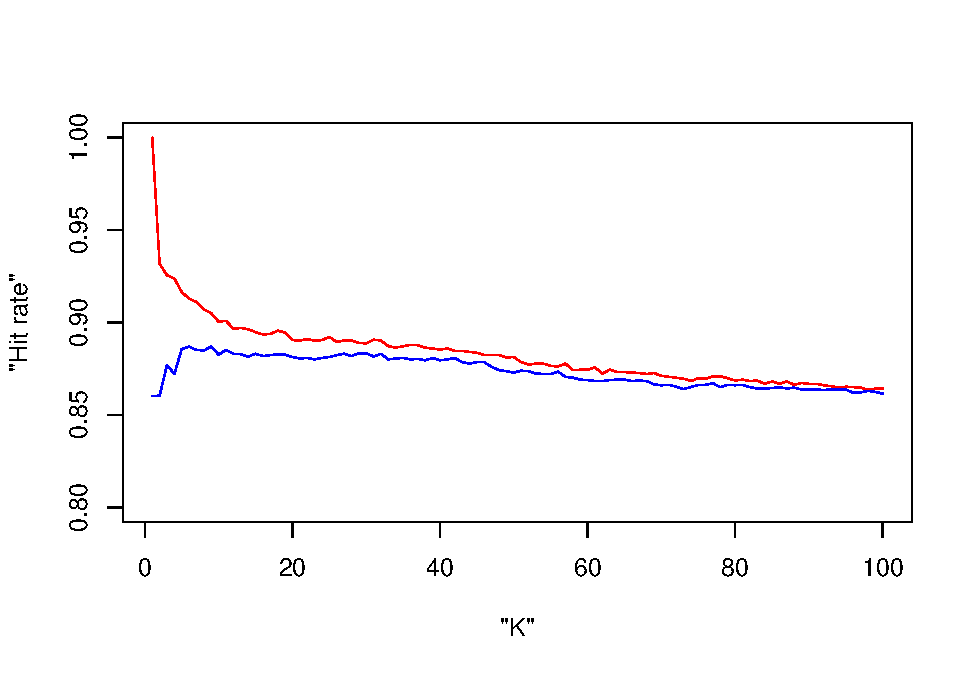
\includegraphics{1_Task_files/figure-latex/Task_1_10-1.pdf}

We can see that with K=1 the model is flexible and by definition, we have training hit rate (red line) of 0, but the LOOCV hit rate (blue line) is higher in this case, while with model less flexible, as with k=98, the two errors are similar.
Since both the errors increase if we increase the parameter K, probably the model that describes the dataset better is the model with K=30 or K=66.

\begin{table}[h!]
  \begin{center}
    \caption{}
    \label{tab:}
    \begin{tabular}{c|c|c} % <-- Alignments: 1st column left, 2nd middle and 3rd right, with vertical lines in between
      \textbf{K} & \textbf{TRAINING HIT RATE} & \textbf{LOOCV HIT RATE}\\
      %\ \alpha$ & $\beta$ & $\gamma$ \\ 
      \hline
      1 & 1 & 0.8601630\\
      30 & 0.8886908 & 0.8833418\\
      66 & 0.8728986 & 0.8683138\\
      100 & 0.8642384 & 0.8614366\\
    \end{tabular}
  \end{center}
\end{table}

\hypertarget{high-dimensional-discriminant-analysis}{%
\subsection{High Dimensional Discriminant Analysis}\label{high-dimensional-discriminant-analysis}}

The fourth method that we have used to discriminate between different groups is the HDDA method. This method could be useful while the number of parameters is high compared to the number of data.

\begin{Shaded}
\begin{Highlighting}[]
\NormalTok{w }\OtherTok{\textless{}{-}}\NormalTok{ dwvs[,}\SpecialCharTok{{-}}\DecValTok{1}\NormalTok{]}
\NormalTok{cls }\OtherTok{\textless{}{-}}\NormalTok{ dwvs[,}\DecValTok{1}\NormalTok{]}
\CommentTok{\#HDDA on the learning dataset:}
\NormalTok{hdda.out7 }\OtherTok{\textless{}{-}} \FunctionTok{hdda}\NormalTok{(w, cls, }\AttributeTok{scaling=}\ConstantTok{TRUE}\NormalTok{, }\AttributeTok{model=}\StringTok{"all"}\NormalTok{, }\AttributeTok{d=}\StringTok{"BIC"}\NormalTok{,}\AttributeTok{graph=}\ConstantTok{TRUE}\NormalTok{,}\AttributeTok{show=}\ConstantTok{TRUE}\NormalTok{) }
\end{Highlighting}
\end{Shaded}

\begin{verbatim}
 # :     Model     BIC
 1 :     AKJBKQKDK   -67912.32  
 2 :     AKBKQKDK    -68249.76  
 3 :     ABKQKDK     -69185.72  
 4 :     AKJBQKDK    -69646.01  
 5 :     AKBQKDK     -69983.46  
 6 :     ABQKDK      -70919.41  
 7 :     AKJBKQKD    -67492.38  
 8 :     AKBKQKD     -68372.73  
 9 :     ABKQKD      -68803.13  
10 :     AKJBQKD     -68044.89  
11 :     AKBQKD      -68925.24  
12 :     ABQKD       -69355.63  
13 :     AJBQD       -71078.02  
14 :     ABQD        -71609.34  

SELECTED: Model AKJBKQKD, BIC=-67492.38.
\end{verbatim}

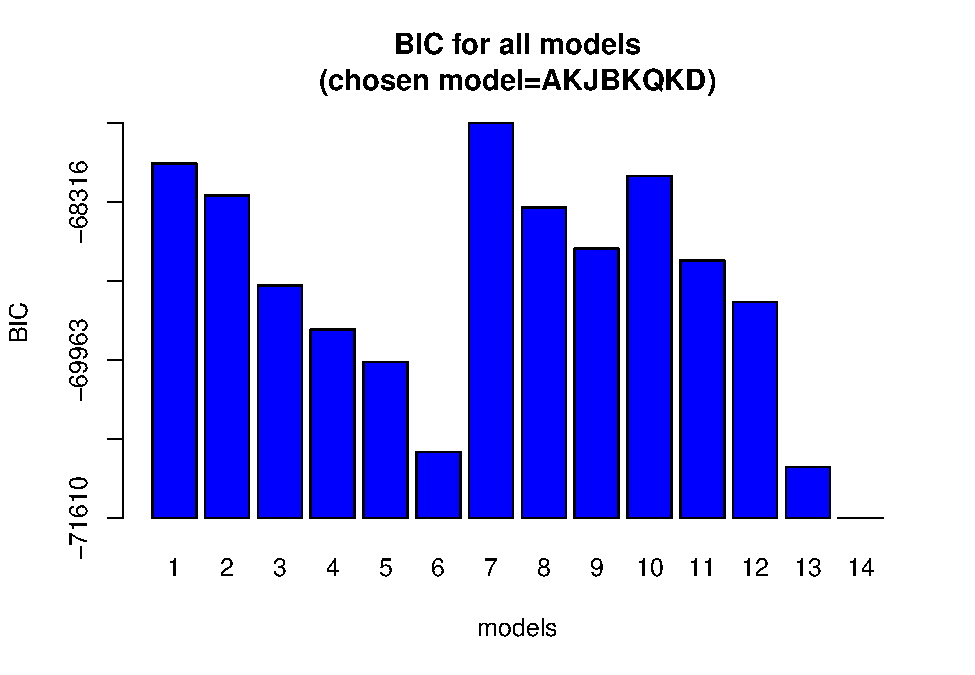
\includegraphics{1_Task_files/figure-latex/Task_1_11-1.pdf}

\begin{Shaded}
\begin{Highlighting}[]
\FunctionTok{plot}\NormalTok{(hdda.out7)}
\end{Highlighting}
\end{Shaded}

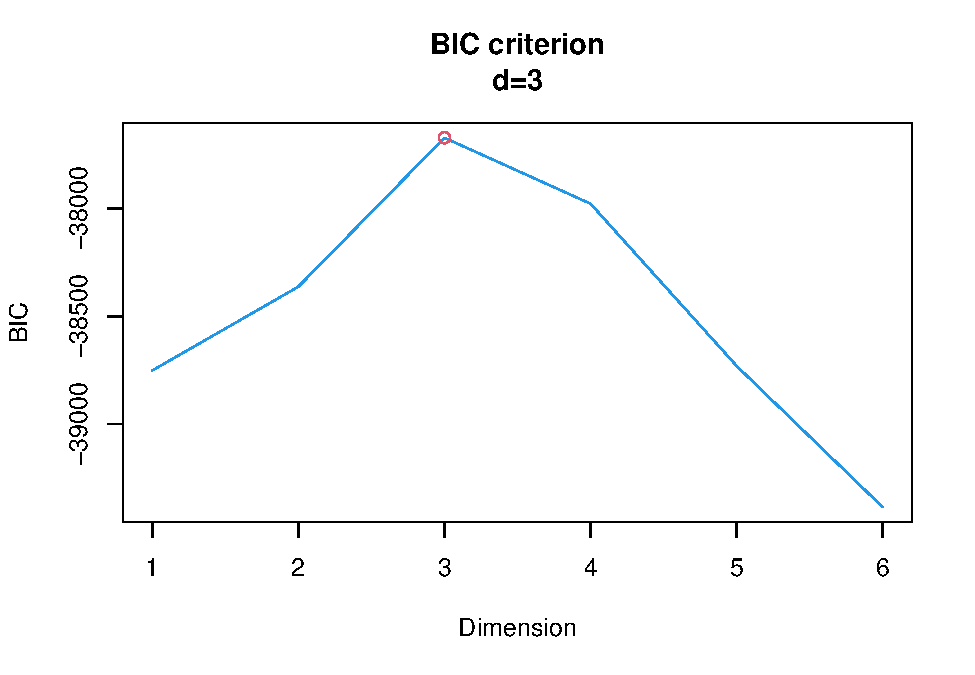
\includegraphics{1_Task_files/figure-latex/Task_1_11-2.pdf}

The model used from the HDDA analysis applying the BIC criterion is model \(7(A_{kj} K_{j} B_{k} Q_{k} d)\). The decision following the \emph{BIC} criteria is to choose the model with the lowest value, in that case, the reference system is negative, so the lowest value is for model \(7\).

\begin{Shaded}
\begin{Highlighting}[]
\FunctionTok{plot}\NormalTok{(hdda.out7,}\AttributeTok{method=}\StringTok{"BIC"}\NormalTok{)}
\end{Highlighting}
\end{Shaded}

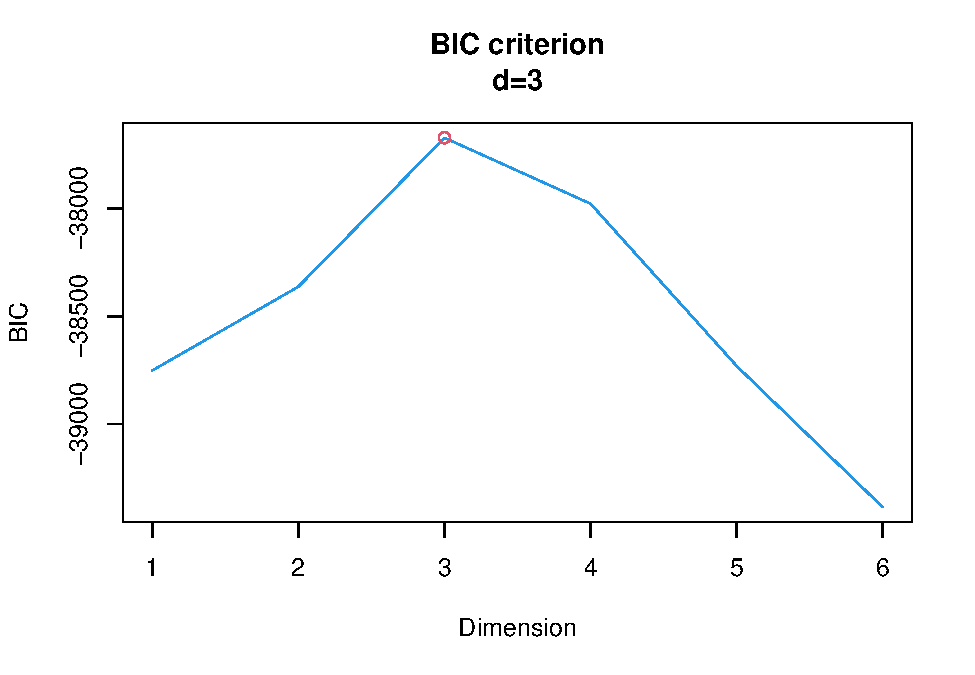
\includegraphics{1_Task_files/figure-latex/Task_1_12-1.pdf}

The dimension choose for the model is \(3\). The model chosen by the \emph{BIC} criteria has the same number of principal components for all the three different classes.

\begin{Shaded}
\begin{Highlighting}[]
\NormalTok{pred.train7}\OtherTok{\textless{}{-}}\FunctionTok{predict}\NormalTok{(hdda.out7,w,cls)}
\end{Highlighting}
\end{Shaded}

\begin{verbatim}
Correct classification rate: 0.8530311.
               Initial class
Predicted class Netherlands Nigeria Philippines
    Netherlands        1196      20          40
    Nigeria              26    1356         251
    Philippines          38     202         797
\end{verbatim}

\begin{Shaded}
\begin{Highlighting}[]
\CommentTok{\#print(tab7)}
\NormalTok{tab7}\OtherTok{\textless{}{-}}\FunctionTok{table}\NormalTok{(dwvs}\SpecialCharTok{$}\NormalTok{country,pred.train7}\SpecialCharTok{$}\NormalTok{class)}
\CommentTok{\#training hit rate}
\FunctionTok{kbl}\NormalTok{(}\FunctionTok{sum}\NormalTok{(}\FunctionTok{diag}\NormalTok{(tab7))}\SpecialCharTok{/}\FunctionTok{sum}\NormalTok{(tab7))}
\end{Highlighting}
\end{Shaded}

\begin{tabular}[t]{r}
\hline
x\\
\hline
0.8530311\\
\hline
\end{tabular}

\begin{Shaded}
\begin{Highlighting}[]
\NormalTok{pred.loocv8 }\OtherTok{\textless{}{-}} \FunctionTok{hdda}\NormalTok{(w, cls,}\AttributeTok{scaling=}\ConstantTok{TRUE}\NormalTok{, }\AttributeTok{d=}\StringTok{"BIC"}\NormalTok{, }\AttributeTok{LOO=}\ConstantTok{TRUE}\NormalTok{)}
\NormalTok{tab8}\OtherTok{\textless{}{-}}\FunctionTok{table}\NormalTok{(cls,pred.loocv8}\SpecialCharTok{$}\NormalTok{class)}
\CommentTok{\#print(tab8)}
\FunctionTok{kbl}\NormalTok{(tab8)}
\end{Highlighting}
\end{Shaded}

\begin{tabular}[t]{l|r|r|r}
\hline
  & Netherlands & Nigeria & Philippines\\
\hline
Netherlands & 1197 & 26 & 37\\
\hline
Nigeria & 22 & 1378 & 178\\
\hline
Philippines & 44 & 285 & 759\\
\hline
\end{tabular}

\begin{Shaded}
\begin{Highlighting}[]
\CommentTok{\#LOOCV hit rate}
\FunctionTok{kbl}\NormalTok{(}\FunctionTok{sum}\NormalTok{(}\FunctionTok{diag}\NormalTok{(tab8))}\SpecialCharTok{/}\FunctionTok{sum}\NormalTok{(tab8))}
\end{Highlighting}
\end{Shaded}

\begin{tabular}[t]{r}
\hline
x\\
\hline
0.8492104\\
\hline
\end{tabular}

Also with the \emph{HDDA} model, there is rather small evidence of overfitting, but the HDDA model does not perform better than the other models.

\hypertarget{error-comparison-for-the-different-models}{%
\subsection{Error comparison for the different models}\label{error-comparison-for-the-different-models}}

We have computed for all 4 models the hit rate, for the comparison in the table we will present the training and LOOCV errors computing \(1-*hit\) rate:

\begin{table}[h!]
  \begin{center}
  \caption{}
    \begin{tabular}{c|c|c} 
      \textbf{MODEL} & \textbf{TRAINING ERROR} & \textbf{LOOCV ERROR}\\
      \hline
        LDA & 0.1535914 & 0.154865\\
        QDA & 0.1449312 & 0.1474783\\
        KNN (K=30) & 0.1113092 & 0.1166582\\
        HDDA & 0.1469689 & 0.1507896\\
      \end{tabular}
    \end{center}
\end{table}

In all the present models there is little evidence of overfitting, the two errors computed are in all the cases similar. The K-nearest Neighbors is a good model to compare the others and we can see that even if it performs betters it has not a huge difference. The model that performs better between the other \(3\) is the Quadratic discriminant analysis, it is the most complex one with the highest number of parameters used.

Confronting the results, we can say that even if there is a difference between the models, no one of the computed ones has outstanding results.

Table of \emph{QDA LOOCV} rate:

\begin{table}[h!]
  \begin{center}
    \caption{}
      \begin{tabular}{c|c|c|c} 
      \textbf{ - } & \textbf{Netherlands} & \textbf{Nigeria} & \textbf{Philippines}\\
      \hline
        Netherlands & 1210 & 21 & 29\\
        Nigeria & 40 & 1315 & 223\\
        Philippines & 43 & 223 & 822\\
    \end{tabular}
  \end{center}
\end{table}

As we were expecting in the analysis of the canonical discriminant analysis, the model has a high ability to differentiate between Netherlands and the two other countries, while it has a high error rate discriminating between Nigeria and the Philippines.

\hypertarget{multinomial-logistic-regression-model}{%
\subsection{Multinomial logistic regression model}\label{multinomial-logistic-regression-model}}

\begin{Shaded}
\begin{Highlighting}[]
\NormalTok{m1}\OtherTok{\textless{}{-}} \FunctionTok{multinom}\NormalTok{(country}\SpecialCharTok{\textasciitilde{}}\NormalTok{F\_rights}\SpecialCharTok{+}\NormalTok{F\_steal}\SpecialCharTok{+}\NormalTok{F\_crime}\SpecialCharTok{+}\NormalTok{F\_religion}\SpecialCharTok{+}\NormalTok{F\_realizeself}\SpecialCharTok{+}\NormalTok{F\_dogood }\SpecialCharTok{+}
\NormalTok{                F\_violence, }\AttributeTok{family=}\NormalTok{multinomial, }\AttributeTok{data=}\NormalTok{dwvs, }\AttributeTok{maxit=}\DecValTok{3926}\NormalTok{, }\AttributeTok{hess=}\ConstantTok{TRUE}\NormalTok{)}
\end{Highlighting}
\end{Shaded}

\begin{verbatim}
# weights:  27 (16 variable)
initial  value 4313.151845 
iter  10 value 1376.724330
iter  20 value 1352.584896
final  value 1346.617148 
converged
\end{verbatim}

\begin{Shaded}
\begin{Highlighting}[]
\NormalTok{t1\_15\_result }\OtherTok{\textless{}{-}} \FunctionTok{summary}\NormalTok{ (m1)}
\NormalTok{t1\_15\_result}
\end{Highlighting}
\end{Shaded}

\begin{verbatim}
Call:
multinom(formula = country ~ F_rights + F_steal + F_crime + F_religion + 
    F_realizeself + F_dogood + F_violence, data = dwvs, family = multinomial, 
    maxit = 3926, hess = TRUE)

Coefficients:
            (Intercept)  F_rights   F_steal   F_crime F_religion F_realizeself
Nigeria       0.6472240 -2.122889 0.5537755 0.5976742   2.887712     2.8922393
Philippines   0.9959826 -1.466848 1.5556448 1.0662700   1.932117     0.9680894
               F_dogood F_violence
Nigeria     -0.01110756  1.2844737
Philippines  1.16765772  0.7560728

Std. Errors:
            (Intercept)  F_rights   F_steal   F_crime F_religion F_realizeself
Nigeria       0.1612100 0.1642741 0.1735127 0.1334749  0.2143403     0.1695936
Philippines   0.1510987 0.1475679 0.1685630 0.1296852  0.1866007     0.1556415
             F_dogood F_violence
Nigeria     0.1218099  0.1534901
Philippines 0.1197516  0.1470007

Residual Deviance: 2693.234 
AIC: 2725.234 
\end{verbatim}

We can see that there are 2 different regression model estimates: the first one compares the probability of Nigeria to the probability of the Netherlands, the second model compares the probability of the Philippines to the probability of the Netherlands.
All the parameters are significant except \emph{F\_dogood} for Nigeria, which's not significantly different from 0.
The sign of the parameters is the same for all the parameters in both the regressions, except for \emph{F\_dogood} where the Nigeria coefficient is not significant. This could be explained because have we analyzed previously Netherlands strongly differs from the other two countries, while Nigeria and the Philippines have not a clear separation.
This analysis shows that sample data is more likely to belong to Nigeria and the Philippines than to the Netherlands when it has a higher positive value in the parameters of steal, crime, violence, religion, and a lower negative value in rights
These coefficients could be probably well explained from the fact that the Netherlands is one of the most developed countries in all the world, the statistics of the Human Development Index published by the United Nations Development Programme places it in the 8th place in the world, while Nigeria and the Philippines are both considered developing states (161 and 107 respectively in the HDI ranking).

\begin{Shaded}
\begin{Highlighting}[]
\DocumentationTok{\#\#\#\# compute hitrate training data\#\#\#\#}
\NormalTok{train.pred}\OtherTok{\textless{}{-}}\FunctionTok{predict}\NormalTok{(m1,}\AttributeTok{newdata=}\NormalTok{dwvs)}
\NormalTok{tab}\OtherTok{\textless{}{-}}\FunctionTok{table}\NormalTok{(dwvs}\SpecialCharTok{$}\NormalTok{country, train.pred)}
\FunctionTok{kbl}\NormalTok{(}\FunctionTok{sum}\NormalTok{(}\FunctionTok{diag}\NormalTok{(tab))}\SpecialCharTok{/}\FunctionTok{sum}\NormalTok{(tab))}
\end{Highlighting}
\end{Shaded}

\begin{tabular}[t]{r}
\hline
x\\
\hline
0.8571065\\
\hline
\end{tabular}

Error rate: 0.1428935

\begin{Shaded}
\begin{Highlighting}[]
\DocumentationTok{\#\#\#\#\#\#\#\#compute LOOCV}
\NormalTok{nobs}\OtherTok{\textless{}{-}} \DecValTok{3926}
\NormalTok{hit}\OtherTok{\textless{}{-}}\FunctionTok{rep}\NormalTok{(}\DecValTok{0}\NormalTok{,nobs)}
\ControlFlowTok{for}\NormalTok{ (i }\ControlFlowTok{in} \DecValTok{1}\SpecialCharTok{:}\NormalTok{nobs)\{}
\NormalTok{  train}\OtherTok{\textless{}{-}}\FunctionTok{c}\NormalTok{(}\DecValTok{1}\SpecialCharTok{:}\NormalTok{nobs)}
\NormalTok{  mod}\OtherTok{\textless{}{-}} \FunctionTok{multinom}\NormalTok{(country }\SpecialCharTok{\textasciitilde{}}\NormalTok{ F\_rights }\SpecialCharTok{+}\NormalTok{ F\_steal }\SpecialCharTok{+}\NormalTok{ F\_crime }\SpecialCharTok{+}\NormalTok{ F\_religion }\SpecialCharTok{+} 
\NormalTok{                   F\_realizeself }\SpecialCharTok{+}\NormalTok{ F\_dogood }\SpecialCharTok{+}\NormalTok{ F\_violence, }\AttributeTok{data=}\NormalTok{dwvs, }
                 \AttributeTok{subset=}\NormalTok{train[}\SpecialCharTok{{-}}\NormalTok{i], }\AttributeTok{print=} \ConstantTok{FALSE}\NormalTok{,}\AttributeTok{maxit=}\DecValTok{3926}\NormalTok{)}
\NormalTok{  pred}\OtherTok{\textless{}{-}} \FunctionTok{predict}\NormalTok{(mod, }\AttributeTok{newdata=}\NormalTok{dwvs[i,])}
\NormalTok{  hit[i]}\OtherTok{\textless{}{-}}\FunctionTok{ifelse}\NormalTok{(pred}\SpecialCharTok{==}\NormalTok{dwvs}\SpecialCharTok{$}\NormalTok{country[i],}\DecValTok{1}\NormalTok{,}\DecValTok{0}\NormalTok{)}
\NormalTok{\}}
\end{Highlighting}
\end{Shaded}

\begin{Shaded}
\begin{Highlighting}[]
\CommentTok{\#hitrate}
\FunctionTok{mean}\NormalTok{(hit)  }\DocumentationTok{\#\#\#\# LOOCV}
\end{Highlighting}
\end{Shaded}

Error rate: 0.1444218

The Multinomial logistic regression model has slightly better error values than the other models, except for KNN.

\end{document}
